%----------------------------------------------------------------------------
\chapter{Graph Engine}
%----------------------------------------------------------------------------

A Graph Engine a Microsoft cég egyik projektje, amit 2010. október 30-án indítottak el, akkor még \emph{Trinity} néven. Ez egy gráfadatbázis-rendszer ami memóriafelhőn fut. A memóriafelhő egy globálisan címezhető, memóriában található kulcs-érték tároló. Mivel memóriaalapú, ezért gyors véletlen elérést biztosít nagyméretű gráfok esetén is, támogatja a gyors gráfbejárást és a párhuzamos feldolgozást is.

Az elkészített megoldás Microsoft Windows 7 x64 operációs rendszeren, Visual Studioban készült és \Csh{} nyelven, ezért a továbbiakban leírtak erre a környezetre vonatkoznak.


\section{A Graph Engine felépítése}

\section{\emph{TSL}}

A \emph{TSL}, azaz \emph{Trinity Specification Language} a Graph Engine gráfséma-leíró nyelve. Az előre definiált adatstruktúra helyett nagy könnyebbséget kínál azáltal, hogy szerveroldalon az adott alkalmazásra specifikus adatstruktúrát adhatunk meg. Szintaxisát tekintve leginkább a C, \cpp{}  és a \Csh{} nyelvre hasonlít.

A \emph{TSL} lehetőséget kínál sokfajta beépített típus használatára, melyek a következők:
\begin{itemize}
	\item \texttt{bool} \--- logikai
	\item \texttt{char} \--- karakter
	\item \texttt{int8, uint8, int16, uint16, int32, uint32, int64, uint64} \--- egész szám 
		
		Az \texttt{u} azt jelöli, hogy előjel nélküli, a szám pedig azt, hogy hány bites.
	\item \texttt{CellId} \--- 64 bites előjeles egész szám
		
		A különbség a \texttt{Cellid} és az \texttt{int64} között a programozó irányába hordozott jelentésben van. A \texttt{CellId}-t cellák egyedi azonosítójára való hivatkozásra használják.
	\item \texttt{float, double} \--- lebegőpontos szám
		A \texttt{float} 32, a \texttt{double} 64 bites.
	\item \texttt{decimal} \--- fix pontosságú szám 128 biten tárolva
	\item \texttt{DateTime} \--- dátum
	\item \texttt{Guid} \--- 128 bites egyedi azonosító
\end{itemize}

A Graph Engine egy ilyen \emph{TSL} fájl alapján építi fel az adatbázis sémáját. Ennek a fájlnak a kiterjesztési \emph{.tsl} és a következő elemekből épül fel:
\begin{itemize}
	\item \texttt{include \ldots{}} \--- Az \emph{include} után megadott fájlt ennek a fájlnak az elejére fűzi.
	\item \texttt{enum\{\ldots{} \}} \--- Felsorolás típust írhatunk le benne hasonlóan, mint C-ben.
	\item \texttt{struct structNeve \{\ldots{} \}} \--- Személyre szabható típus. Beépített típusok, konténerek és más \texttt{struct}-ok helyezhetőek el benne. A \emph{TSL} háromféle konténer típust támogat:
	\begin{itemize}
		\item \texttt{Array<T>} \--- T típusú elemek tömbje. Csak beépített típust támogat.
		\item \texttt{List<T>} \--- T típusú elemek listája. Előnye a tömbbel szemben, hogy dinamikus méretű elemek (konténerek) is tárolhatóak benne. A \Csh{}-ban lévő \texttt{List<T>}-nek megfeleltethető.
		 \item \texttt{string} \--- Karakterek sorozatát lehet benne tárolni.
	\end{itemize}
	\item \texttt{cell cellaNeve\{\ldots{} \}} \--- Struktúráját tekintve hasonló a \texttt{struct} típushoz, ellenben minden \texttt{cell}-hez tartozik egy egyedi azonosító (\texttt{CellId}), amin keresztül hivatkozni lehet rá. 
	\item Attribútumok \--- Stringek kulcs-érték párosa. Segítségükkel futási idejű információt lehet adni az adott celláról vagy mezőjéről.
	\item \texttt{protocol, server, proxy} \--- Távoli adatbázis-elérést lehet velük konfigurálni.
\end{itemize}

A \emph{TSL}-t külön projektbe kell elhelyezni. Fordítása után egy \emph{dll} könyvtár jön létre, amit a másik \Csh{} projektünkhöz hozzálinkelhetünk. Amennyiben a Graph Engine beépített projektjét használjuk és egy \emph{solution} alatt dolgozunk, akkor ezt a Visual Studio elvégzi helyettünk. 

\subsection{Példa \emph{TSL} fájlra}

A példában egy baráti társaságban lévő emberekről tárolunk adatokat. Ezek az adatok legyenek a következők minden embernél: név, személyiigazolvány-szám, barátok. Sokféle megoldás létezhet ennek a problémának a leírására, mivel a nevet tárolhatjuk egy \texttt{string}-ben, de akár egy struktúrában is, a személyiigazolvány-szám lehet fix hosszúságú 6 karakter vagy lehet egy változó hosszú \texttt{string}. Esetünkben a név egy struktúra, a  személyiigazolvány-szám pedig \texttt{string} típusú.

\begin{figure}[ht!]
	\centering
	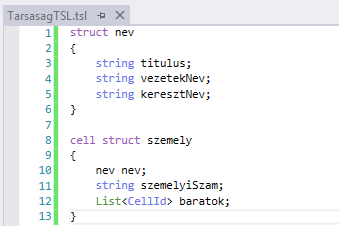
\includegraphics[]{figures/TarsasagTSL.png}
	\caption{Példa TSL használatára.}
	\label{fig:TSL}
\end{figure}

\section{Adatelérés}

A Graph Engine fordítás után a \texttt{cell} típushoz készít úgynevezett \emph{Accessor}-okat, melyek az adatolvasást és manipulálást könnyítik meg. Ezzel párhuzamosan létrehoz osztályokat, amiket a Visual Studioban lévő IntelliSense is tud kezelni, megkönnyítve a további implementációs munkát. Az \emph{Accessor}-okon keresztül 

\subsection{\emph{LINQ}}

\subsection{\emph{LIKQ}}

\section{Példaalkalmazás}